\documentclass[12pt,a4paper]{article}

\usepackage{fontspec}
\usepackage{polyglossia}
\setmainlanguage{russian}
\setotherlanguage{english}
\setmainfont{Times New Roman}[Ligatures=TeX]
\setmonofont{Courier New}
\newfontfamily\cyrillicfont{Times New Roman}[Ligatures=TeX]
\newfontfamily\cyrillicfonttt{Courier New}
\newfontfamily\cyrillicfontsf{Times New Roman}
\usepackage{amsmath,amssymb}
\usepackage{geometry}
\usepackage{graphicx}
\usepackage[hidelinks]{hyperref}
\usepackage{xurl}
\usepackage{microtype}
\usepackage{booktabs}
\usepackage{array}
\usepackage{setspace}
\usepackage{indentfirst}
\usepackage{fancyhdr}
\usepackage{caption}
\usepackage{listings}
\usepackage{xcolor}
\usepackage{float}

\geometry{left=30mm, right=15mm, top=20mm, bottom=20mm, headheight=15pt}
\onehalfspacing
\setlength{\parindent}{1.25cm}
\emergencystretch=3em

\pagestyle{fancy}
\fancyhf{}
\fancyfoot[C]{\thepage}
\renewcommand{\headrulewidth}{0pt}

\makeatletter
\renewcommand\section{\@startsection{section}{1}{\z@}%
  {12pt}{6pt}{\normalfont\normalsize\bfseries}}
\renewcommand\subsection{\@startsection{subsection}{2}{\z@}%
  {10pt}{4pt}{\normalfont\normalsize\bfseries}}
\renewcommand\subsubsection{\@startsection{subsubsection}{3}{\z@}%
  {8pt}{4pt}{\normalfont\normalsize\bfseries}}
\makeatother

\captionsetup[figure]{labelsep=endash, justification=centering, font={onehalfspacing}}
\captionsetup[table]{labelsep=endash, justification=raggedright, singlelinecheck=false, font={onehalfspacing}}

\lstset{
    basicstyle=\ttfamily\footnotesize,
    breaklines=true,
    columns=flexible,
    keepspaces=true,
    showstringspaces=false,
    frame=single,
    framesep=2pt,
    xleftmargin=4pt,
    xrightmargin=4pt,
}

\begin{document}

% названия структурных элементов (переопределяем после polyglossia)
\renewcommand{\contentsname}{СОДЕРЖАНИЕ}
\renewcommand{\figurename}{Рисунок}
\renewcommand{\tablename}{Таблица}

% нумерация разделов без завершающей точки (как в шаблоне)
\makeatletter
\renewcommand{\thesection}{\arabic{section}}
\renewcommand{\thesubsection}{\thesection.\arabic{subsection}}
\renewcommand{\thesubsubsection}{\thesubsection.\arabic{subsubsection}}
\renewcommand\@seccntformat[1]{\csname the#1\endcsname\quad}
\makeatother

% ======== ТИТУЛЬНАЯ СТРАНИЦА ========
\begin{titlepage}
\thispagestyle{empty}
\begin{center}
Правительство Российской Федерации\\
ФЕДЕРАЛЬНОЕ ГОСУДАРСТВЕННОЕ АВТОНОМНОЕ\\
ОБРАЗОВАТЕЛЬНОЕ УЧРЕЖДЕНИЕ ВЫСШЕГО ОБРАЗОВАНИЯ\\
<<НАЦИОНАЛЬНЫЙ ИССЛЕДОВАТЕЛЬСКИЙ УНИВЕРСИТЕТ\\
<<ВЫСШАЯ ШКОЛА ЭКОНОМИКИ>>\\
(НИУ ВШЭ)\\[4pt]
Московский институт электроники и математики им.\,А.\,Н.\,Тихонова\\[40pt]

{\large \textbf{ОТЧЕТ}}\\[4pt]
{\large О ПРАКТИЧЕСКОЙ РАБОТЕ № 5}\\[4pt]
по дисциплине <<Основы криптографии и стеганографии>>\\[10pt]
\textbf{Встраивание цифровых водяных знаков в частотную область цифровых изображений (гибридный алгоритм ДКП и ДВП)}\\[50pt]
\end{center}

\begin{flushright}
\begin{minipage}{0.45\textwidth}
\raggedright
Студент гр. БИБ254\\
\_\_\_\_\_\_\_\_\_\_\_\_\_ А.\,О.\,Манин\\[8pt]
<<\_\_\_>> \_\_\_\_\_\_\_\_\_ 2026~г.\\[20pt]
Руководитель\\
Заведующий кафедрой информационной\\
безопасности киберфизических систем\\
канд. техн. наук, доцент\\
\_\_\_\_\_\_\_\_\_\_\_\_\_\_О.\,О.\,Евсютин\\[8pt]
<<\_\_\_>> \_\_\_\_\_\_\_\_\_\_ 2026~г.
\end{minipage}
\end{flushright}

\vfill
\begin{center}
Москва 2026
\end{center}
\end{titlepage}

% ======== СОДЕРЖАНИЕ ========
\tableofcontents
\newpage

% ================================================================
\section{Задание на практическую работу}

Целью работы является приобретение навыков программной реализации алгоритмов встраивания цифровых водяных знаков (ЦВЗ) в частотную область цифровых изображений.

В рамках практической работы необходимо выполнить следующее:
\begin{enumerate}
    \item написать программную реализацию одного из двух рассмотренных методов встраивания ЦВЗ в частотную область цифровых изображений по выбору студента. В данной работе выбран гибридный алгоритм на основе дискретного косинусного преобразования (ДКП) и дискретного вейвлет-преобразования (ДВП)~[2];
    \item провести вычислительные эксперименты с полученной программной реализацией и сделать выводы об эффективности рассмотренного метода встраивания;
    \item подготовить отчет о выполнении работы.
\end{enumerate}

Программа должна обладать следующей функциональностью:
\begin{enumerate}
    \item при встраивании: принимать на вход изображение-контейнер и ЦВЗ для встраивания, рассчитывать показатели качества встраивания;
    \item при извлечении: принимать на вход изображение, содержащее ЦВЗ, и при необходимости исходное изображение-контейнер;
    \item осуществлять встраивание или извлечение информации по выбору пользователя.
\end{enumerate}

Вычислительные эксперименты должны включать оценку незаметности встраивания и оценку робастности~--- извлечение ЦВЗ в условиях отсутствия атак и при наличии нескольких типичных атак (обязательно JPEG-сжатие с несколькими степенями сжатия). При оценке незаметности и робастности должна быть учтена зависимость данных показателей от параметров алгоритма встраивания.

% ================================================================
\section{Краткая теоретическая часть}

\subsection{Цифровые водяные знаки и частотные методы встраивания}

Цифровой водяной знак~--- это дополнительная информация, встраиваемая в цифровое изображение с целью его аутентификации или контроля целостности. По степени устойчивости к искажениям различают \textit{хрупкие} ЦВЗ (разрушаются при любом изменении контейнера), \textit{полухрупкие} (выдерживают разрешенные преобразования) и \textit{робастные} (обнаружимы даже после существенных искажений)~[1]. Наибольшую практическую ценность для защиты авторства имеют робастные ЦВЗ, сохраняющиеся после типичных операций обработки изображений: кадрирования, масштабирования, изменения яркости и JPEG-сжатия.

Встраивание в частотную область, как правило, обеспечивает большую робастность при сохранении визуальной незаметности, чем встраивание в пространственную область. Идея состоит в том, чтобы применить к изображению некоторое частотное преобразование (ДКП, ДПФ, ДВП) и изменить полученные частотные коэффициенты. Энергия встраиваемого знака распределяется по множеству пикселей, поэтому локальные искажения (в т.ч. вносимые сжатием) не разрушают ЦВЗ полностью.

\subsection{Гибридный алгоритм встраивания ЦВЗ на основе ДКП и ДВП}

В работе реализован гибридный алгоритм~[2], сочетающий ДКП и ДВП. В качестве контейнера используется полутоновое квадратное изображение разрешением $N \times N$; ЦВЗ~--- бинарное изображение разрешением $m \times m$, $m < N$. Извлечение является \textit{неслепым}: на этапе извлечения требуется как изображение со встроенным ЦВЗ, так и исходное изображение-контейнер.

\textbf{Встраивание.} Алгоритм состоит из следующих шагов.
\begin{enumerate}
    \item Ко всему изображению-контейнеру применяется ДКП, в результате чего получается массив коэффициентов $C = \mathrm{DCT}(I)$.
    \item К массиву $C$ применяется один уровень ДВП Хаара, дающий четыре частотных поддиапазона $\mathrm{LL}$, $\mathrm{HL}$, $\mathrm{LH}$, $\mathrm{HH}$ размером $\tfrac{N}{2} \times \tfrac{N}{2}$ каждый.
    \item ЦВЗ перемешивается преобразованием Арнольда, после чего к нему применяется ДКП. Полученный массив коэффициентов делится на четыре равных неперекрывающихся блока размером $\tfrac{m}{2} \times \tfrac{m}{2}$.
    \item Каждый блок коэффициентов ДКП водяного знака встраивается в левый верхний угол одного из четырех поддиапазонов ДВП по формуле
    \begin{equation}
        \mathit{ID}^{\,w}_{i,j} = \mathit{ID}_{i,j} + \alpha \cdot W_{i,j},
    \end{equation}
    где $\mathit{ID}_{i,j}$~--- коэффициент ДВП изображения-контейнера, $W_{i,j}$~--- ДКП-коэффициент водяного знака, $\alpha$~--- коэффициент масштабирования (по умолчанию $\alpha = 20$).
    \item К модифицированному массиву коэффициентов применяется обратное ДВП, а затем обратное ДКП. После округления вещественных значений и приведения к диапазону $[0, 255]$ получается изображение со встроенным ЦВЗ.
\end{enumerate}

\textbf{Извлечение.} Для извлечения ЦВЗ к исходному контейнеру и к изображению со встроенным ЦВЗ последовательно применяются ДКП и один уровень ДВП Хаара. Блоки коэффициентов ДКП водяного знака извлекаются из левого верхнего угла каждого из четырех поддиапазонов по формуле
\begin{equation}
    W_{i,j} = \frac{\mathit{ID}^{\,w}_{i,j} - \mathit{ID}^{\,c}_{i,j}}{\alpha},
\end{equation}
где $\mathit{ID}^{\,c}_{i,j}$ и $\mathit{ID}^{\,w}_{i,j}$~--- коэффициенты ДВП контейнера и изображения со встроенным ЦВЗ соответственно. Четыре блока объединяются в одну матрицу, к которой применяется обратное ДКП; затем выполняется обратное преобразование Арнольда и пороговая бинаризация, дающая восстановленный ЦВЗ.

\subsection{Преобразование Арнольда}

Преобразование Арнольда применяется для перемешивания битов ЦВЗ перед встраиванием. Оно изменяет координаты пикселей квадратной матрицы порядка $m$ по формуле
\begin{equation}
    \begin{pmatrix} x' \\ y' \end{pmatrix} =
    \begin{pmatrix} 1 & 1 \\ 1 & 2 \end{pmatrix}
    \begin{pmatrix} x \\ y \end{pmatrix} \bmod m,
\end{equation}
где $x, y$~--- исходные координаты пикселя, $x', y'$~--- новые координаты. Обратное преобразование задается как
\begin{equation}
    \begin{pmatrix} x \\ y \end{pmatrix} =
    \begin{pmatrix} 2 & -1 \\ -1 & 1 \end{pmatrix}
    \begin{pmatrix} x' \\ y' \end{pmatrix} \bmod m.
\end{equation}
Преобразование выполняется в течение заданного числа итераций для усиления перемешивающего эффекта; то же число итераций используется при восстановлении. Перемешивание делает ошибки извлечения пространственно некоррелированными и повышает устойчивость к локальным искажениям (например, кадрированию).

\subsection{Метрики качества встраивания}

\textbf{Незаметность} оценивается метриками MSE, RMSE, PSNR и SSIM. Для контейнера $P$ и изображения со встроенным ЦВЗ $P'$ размером $M \times N$:
\begin{equation}
    \mathrm{MSE} = \frac{1}{MN}\sum_{i=1}^{M}\sum_{j=1}^{N}\bigl(P_{ij} - P'_{ij}\bigr)^2, \qquad \mathrm{RMSE} = \sqrt{\mathrm{MSE}},
\end{equation}
\begin{equation}
    \mathrm{PSNR} = 10\log_{10}\frac{255^2}{\mathrm{MSE}}\quad\text{дБ}.
\end{equation}
SSIM~--- индекс структурного сходства~[4]:
\begin{equation}
    \mathrm{SSIM} = \frac{(2\mu_P\mu_{P'} + K_1)(2\sigma_{PP'} + K_2)}{(\mu_P^2 + \mu_{P'}^2 + K_1)(\sigma_P^2 + \sigma_{P'}^2 + K_2)}.
\end{equation}

\textbf{Качество восстановления ЦВЗ} оценивается коэффициентом битовой ошибки (BER) и нормированной взаимной корреляцией (NCC) между исходным $W$ и извлеченным $\widehat{W}$ водяными знаками:
\begin{equation}
    \mathrm{BER} = \frac{1}{m^2}\sum_{i,j}\bigl[\,W_{ij} \neq \widehat{W}_{ij}\,\bigr], \qquad
    \mathrm{NCC} = \frac{\sum_{i,j} W_{ij}\widehat{W}_{ij}}{\sqrt{\sum_{i,j} W_{ij}^2}\,\sqrt{\sum_{i,j}\widehat{W}_{ij}^2}}.
\end{equation}
Значение $\mathrm{NCC} = 1$ и $\mathrm{BER} = 0$ соответствуют точному восстановлению ЦВЗ.

% ================================================================
\section{Программная реализация}

\subsection{Архитектура программы}

Реализация выполнена на языке Python в виде пакета \texttt{dwtdct/} со следующими модулями:
\begin{enumerate}
    \item \texttt{dwtdct/watermark.py}~--- ядро метода: одноуровневое ДВП Хаара (\texttt{haar\_dwt2}, \texttt{haar\_idwt2}), прямое и обратное преобразования Арнольда (\texttt{arnold\_scramble}, \texttt{arnold\_unscramble}), функции встраивания \texttt{embed} и извлечения \texttt{extract};
    \item \texttt{dwtdct/metrics.py}~--- расчёт метрик \texttt{psnr}, \texttt{mse}, \texttt{rmse}, \texttt{ssim}, \texttt{ber}, \texttt{ncc};
    \item \texttt{dwtdct/cli.py}~--- интерфейс командной строки с подкомандами \texttt{embed} и \texttt{extract};
    \item \texttt{dwtdct/experiments.py}~--- скрипт автоматического запуска всех вычислительных экспериментов и генерации рисунков для отчёта.
\end{enumerate}

Использовались библиотеки \texttt{numpy} (работа с массивами), \texttt{scipy} (полнокадровое ДКП \texttt{scipy.fft.dctn}/\texttt{idctn}), \texttt{Pillow} (ввод-вывод изображений, JPEG-сжатие), \texttt{scikit-image} (стандартное тестовое изображение, метрика SSIM), \texttt{matplotlib} (построение графиков). Одноуровневое ДВП Хаара реализовано непосредственно средствами \texttt{numpy} (ортонормированный базис, коэффициент~$\tfrac{1}{\sqrt{2}}$).

\subsection{Формат данных и параметры встраивания}

Изображение-контейнер обрабатывается как полутоновое (RGB-изображения переводятся в яркостную компоненту) и представляется массивом \texttt{numpy} формы $(N, N)$. ЦВЗ~--- бинарное квадратное изображение $m \times m$ ($m$ четное, $m \le N$). Параметрами встраивания являются коэффициент масштабирования $\alpha$ и число итераций преобразования Арнольда. Они сохраняются в объекте \texttt{EmbedParams} (сериализуется в JSON) и передаются на этап извлечения вместе с исходным контейнером.

\subsection{Алгоритм встраивания}

Псевдокод функции \texttt{embed} (упрощённо):
\begin{lstlisting}[language=Python]
def embed(cover, watermark, alpha=20, arnold_iters=10):
    C = dctn(cover, norm="ortho")          # полнокадровое ДКП контейнера
    LL, HL, LH, HH = haar_dwt2(C)           # один уровень ДВП Хаара

    W = arnold_scramble(watermark, arnold_iters)
    Wd = dctn(W, norm="ortho")              # ДКП перемешанного ЦВЗ
    blocks = split_into_4_quadrants(Wd)     # 4 блока m/2 x m/2
    half = m // 2
    for subband, blk in zip([LL, HL, LH, HH], blocks):
        subband[:half, :half] += alpha * blk

    C2 = haar_idwt2(LL, HL, LH, HH)         # обратное ДВП
    stego = round(idctn(C2, norm="ortho"))  # обратное ДКП
    return clip(stego, 0, 255), params
\end{lstlisting}

Извлечение работает симметрично: к контейнеру и стегоизображению применяются ДКП и ДВП, из левых верхних углов поддиапазонов извлекается разность $(\mathit{ID}^{w} - \mathit{ID}^{c})/\alpha$, четыре блока объединяются, к ним применяется обратное ДКП, обратное преобразование Арнольда и бинаризация по порогу $0{,}5$.

\subsection{Использование программы}

Программа запускается из каталога \texttt{kriptoprak3}:
\begin{lstlisting}[language=bash]
# встраивание ЦВЗ
python -m dwtdct embed   --cover cover.png --watermark wm.png \
                         --stego stego.png --params params.json \
                         --alpha 20 --iters 10

# извлечение ЦВЗ (неслепое: нужен исходный контейнер)
python -m dwtdct extract --stego stego.png --cover cover.png \
                         --params params.json --output recovered.png \
                         --watermark wm.png
\end{lstlisting}
При встраивании на стандартный вывод печатаются метрики незаметности (PSNR, MSE, RMSE, SSIM); при извлечении~--- BER, NCC и доля верно восстановленных битов. Скрипт \texttt{python -m dwtdct.experiments} выполняет полный пакет вычислительных экспериментов и сохраняет рисунки в каталог \texttt{images/}.

\subsection{Пример работы программы}

В качестве контейнера используется стандартное полутоновое изображение <<Cameraman>> ($512 \times 512$); в качестве ЦВЗ~--- бинарный логотип $64 \times 64$ (рисунки~1 и~2). На рисунке~3 показано изображение со встроенным ЦВЗ при параметрах по умолчанию ($\alpha = 20$, 10~итераций Арнольда), визуально неотличимое от контейнера ($\mathrm{PSNR} = 45{,}75$~дБ, $\mathrm{SSIM} = 0{,}9949$). На рисунке~4 приведена карта абсолютной разности контейнера и стегоизображения (амплитуда усилена для наглядности): искажения распределены по всему изображению, что характерно для частотного встраивания.

\begin{figure}[H]
\centering
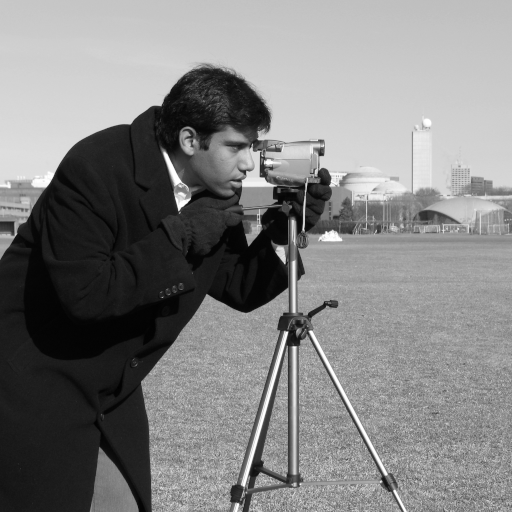
\includegraphics[width=0.45\textwidth,keepaspectratio]{images/cover.png}
\caption{Изображение-контейнер <<Cameraman>> ($512 \times 512$)}
\end{figure}

\begin{figure}[H]
\centering

\includegraphics[width=0.25\textwidth,keepaspectratio]{images/watermark.png}
\caption{Бинарный цифровой водяной знак ($64 \times 64$)}
\end{figure}

\begin{figure}[H]
\centering
\includegraphics[width=0.45\textwidth,keepaspectratio]{images/stego.png}
\hspace{0.5cm}
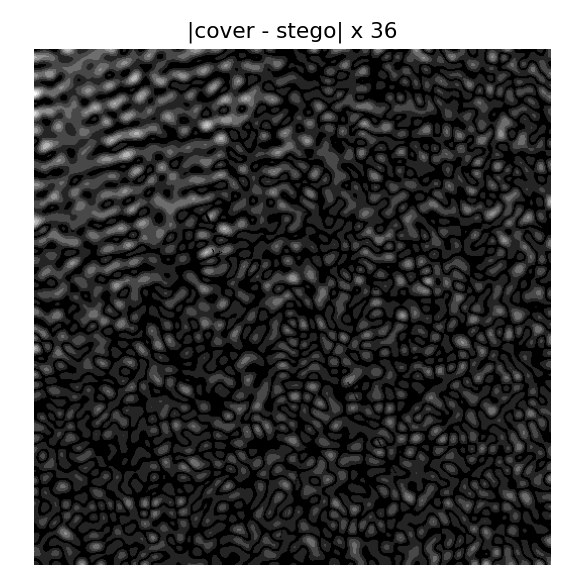
\includegraphics[width=0.45\textwidth,keepaspectratio]{images/diffmap.png}
\caption{Изображение со встроенным ЦВЗ (слева) и карта искажений (справа, амплитуда усилена)}
\end{figure}

При отсутствии атак ЦВЗ восстанавливается без ошибок ($\mathrm{BER} = 0$, $\mathrm{NCC} = 1{,}0$); извлеченный знак приведен на рисунке~5.

\begin{figure}[H]
\centering

\includegraphics[width=0.25\textwidth,keepaspectratio]{images/recovered_clean.png}
\caption{ЦВЗ, извлеченный из стегоизображения при отсутствии атак}
\end{figure}

Корректность пары <<встраивание/извлечение>> проверяется автоматически в скрипте экспериментов: каждый запуск \texttt{embed} сопровождается \texttt{extract} и сравнением восстановленного ЦВЗ с оригиналом.

% ================================================================
\section{Вычислительные эксперименты}

\subsection{Эксперимент 1. Зависимость незаметности от коэффициента $\alpha$}

Коэффициент масштабирования $\alpha$ варьировался в диапазоне от 5 до 60 при фиксированном числе итераций Арнольда (10). Результаты приведены в таблице~1. С ростом $\alpha$ незаметность монотонно ухудшается: $\mathrm{PSNR}$ снижается с 57{,}3~дБ до 36{,}4~дБ, а $\mathrm{SSIM}$~--- с 0{,}9994 до 0{,}9638. Зависимость $\mathrm{PSNR}$ и $\mathrm{SSIM}$ от $\alpha$ показана на рисунке~6.

\begin{flushleft}
Таблица 1~--- Незаметность встраивания при разных значениях $\alpha$
\end{flushleft}
\begin{center}
\begin{tabular}{|p{1.6cm}|p{2.4cm}|p{2.0cm}|p{2.2cm}|p{2.6cm}|}
\hline
\textbf{$\alpha$} & \textbf{PSNR, дБ} & \textbf{MSE} & \textbf{SSIM} & \textbf{BER (без атак)} \\
\hline
5  & 57{,}32 & 0{,}120 & 0{,}9994 & 0{,}0552 \\
\hline
10 & 51{,}22 & 0{,}491 & 0{,}9982 & 0{,}0000 \\
\hline
20 & 45{,}75 & 1{,}732 & 0{,}9949 & 0{,}0000 \\
\hline
30 & 42{,}33 & 3{,}799 & 0{,}9896 & 0{,}0000 \\
\hline
40 & 39{,}88 & 6{,}680 & 0{,}9825 & 0{,}0000 \\
\hline
60 & 36{,}39 & 14{,}92 & 0{,}9638 & 0{,}0000 \\
\hline
\end{tabular}
\end{center}

Следует отметить нетривиальный эффект при $\alpha = 5$: несмотря на наивысшую незаметность, восстановление ЦВЗ даже без атак содержит ошибки ($\mathrm{BER} = 0{,}0552$). Причина~--- округление значений пикселей до целых (\texttt{uint8}) на этапе формирования стегоизображения: при малой силе встраивания вклад ЦВЗ становится сопоставим с шумом квантования и частично теряется. Начиная с $\alpha = 10$, ЦВЗ восстанавливается точно. Таким образом, $\alpha$ нельзя выбирать произвольно малым.

\begin{figure}[H]
\centering
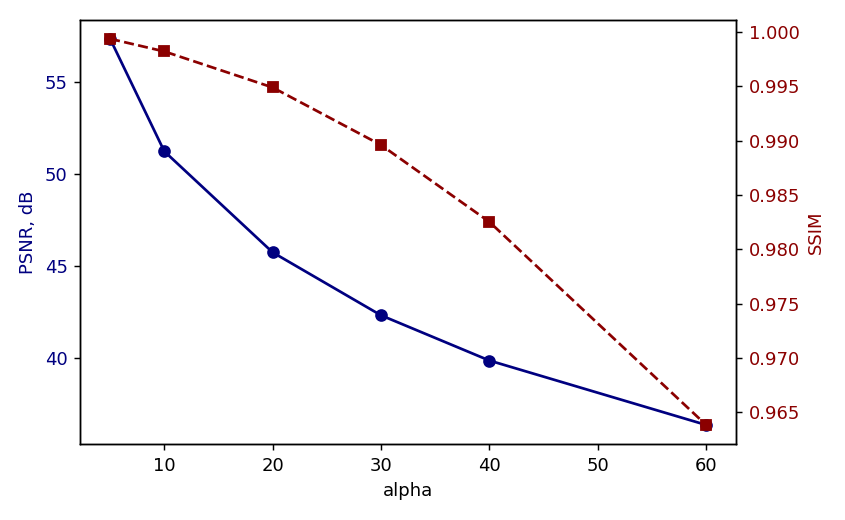
\includegraphics[width=0.7\textwidth,keepaspectratio]{images/psnr_ssim_vs_alpha.png}
\caption{Зависимость PSNR и SSIM от коэффициента масштабирования $\alpha$}
\end{figure}

\subsection{Эксперимент 2. Робастность к типичным атакам}

Стегоизображение, полученное при $\alpha = 20$, подвергалось различным деструктивным воздействиям, после чего проводилось извлечение ЦВЗ. Результаты приведены в таблице~2, а извлеченные водяные знаки~--- на рисунке~7.

\begin{flushleft}
Таблица 2~--- Робастность к атакам ($\alpha = 20$)
\end{flushleft}
\begin{center}
\begin{tabular}{|p{4.5cm}|p{3.0cm}|p{2.2cm}|p{2.2cm}|}
\hline
\textbf{Воздействие} & \textbf{PSNR (стего / обр.), дБ} & \textbf{BER} & \textbf{NCC} \\
\hline
Без атаки & $\infty$ & 0{,}0000 & 1{,}0000 \\
\hline
JPEG $q = 90$ & 40{,}31 & 0{,}0000 & 1{,}0000 \\
\hline
JPEG $q = 70$ & 34{,}32 & 0{,}0002 & 0{,}9995 \\
\hline
JPEG $q = 50$ & 32{,}58 & 0{,}0120 & 0{,}9777 \\
\hline
JPEG $q = 30$ & 31{,}24 & 0{,}1084 & 0{,}8090 \\
\hline
Сдвиг яркости $+20$ & 22{,}13 & 0{,}2063 & 0{,}7416 \\
\hline
Гауссовский шум $\sigma = 5$ & 34{,}19 & 0{,}0264 & 0{,}9516 \\
\hline
Импульсный шум 1\% & 24{,}70 & 0{,}2622 & 0{,}6102 \\
\hline
Масштабирование $0{,}5\times$ & 28{,}21 & 0{,}1023 & 0{,}8295 \\
\hline
Кадрирование 10\% & 8{,}41 & 0{,}4070 & 0{,}3090 \\
\hline
\end{tabular}
\end{center}

Полученные результаты демонстрируют выраженную робастность метода к JPEG-сжатию: при $q = 90$ и $q = 70$ ЦВЗ восстанавливается практически без ошибок ($\mathrm{NCC} \ge 0{,}999$), при $q = 50$ сохраняется высокое качество ($\mathrm{NCC} = 0{,}978$), и даже при сильном сжатии $q = 30$ водяной знак остается визуально читаемым ($\mathrm{NCC} = 0{,}809$). Метод также устойчив к аддитивному гауссовскому шуму ($\mathrm{NCC} = 0{,}952$) и умеренно устойчив к масштабированию ($\mathrm{NCC} = 0{,}830$). Наиболее разрушительными оказались кадрирование ($\mathrm{NCC} = 0{,}309$) и импульсный шум ($\mathrm{NCC} = 0{,}610$): они вносят локальные искажения большой амплитуды, затрагивающие низкочастотные коэффициенты, в которых сосредоточена энергия ЦВЗ. Сдвиг яркости ($\mathrm{NCC} = 0{,}742$) изменяет DC-коэффициент полнокадрового ДКП, что искажает один из коэффициентов ДКП водяного знака и вносит постоянное смещение в часть восстановленного знака.

\begin{figure}[H]
\centering
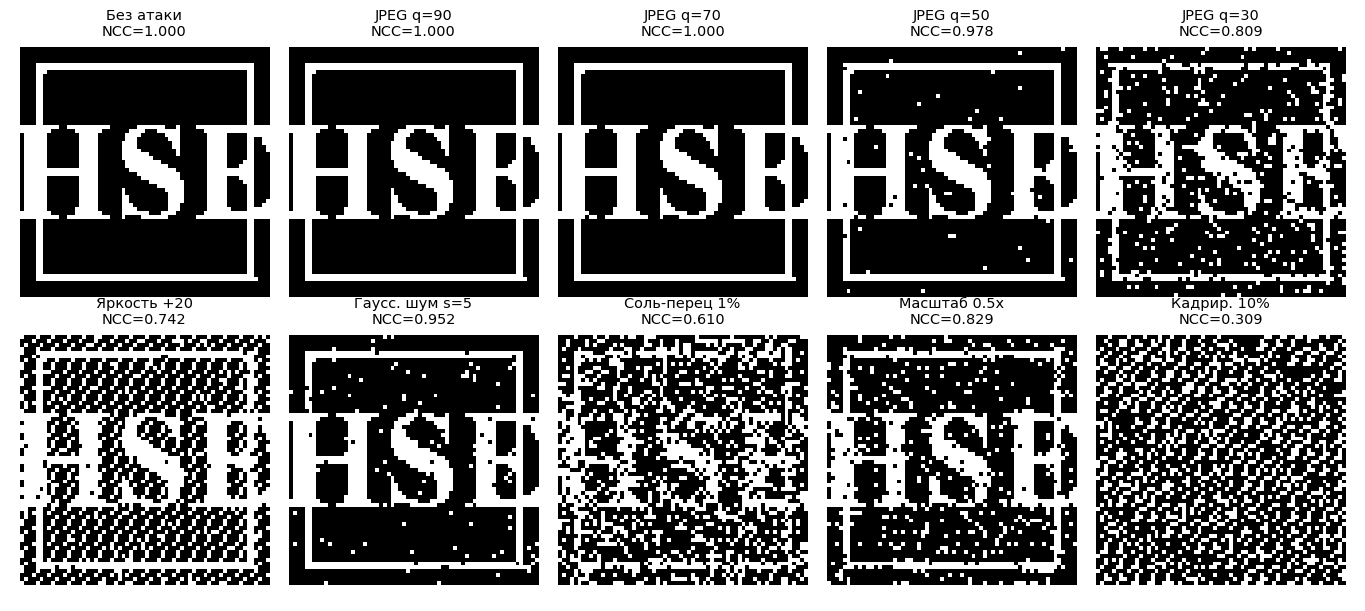
\includegraphics[width=0.98\textwidth,keepaspectratio]{images/recovered_attacks.png}
\caption{ЦВЗ, извлеченные из стегоизображения после различных атак ($\alpha = 20$)}
\end{figure}

\subsection{Эксперимент 3. Зависимость робастности от коэффициента $\alpha$}

Для оценки совместного влияния параметра $\alpha$ на незаметность и робастность стегоизображение, полученное при разных значениях $\alpha$, подвергалось JPEG-сжатию с качеством $q = 50$, после чего извлекался ЦВЗ. Результаты приведены в таблице~3 и на рисунке~8.

\begin{flushleft}
Таблица 3~--- Робастность к JPEG-сжатию ($q = 50$) при разных $\alpha$
\end{flushleft}
\begin{center}
\begin{tabular}{|p{1.6cm}|p{2.4cm}|p{2.4cm}|p{2.4cm}|}
\hline
\textbf{$\alpha$} & \textbf{PSNR, дБ} & \textbf{BER (JPEG)} & \textbf{NCC (JPEG)} \\
\hline
5  & 57{,}32 & 0{,}3330 & 0{,}4868 \\
\hline
10 & 51{,}22 & 0{,}1328 & 0{,}7731 \\
\hline
20 & 45{,}75 & 0{,}0120 & 0{,}9777 \\
\hline
30 & 42{,}33 & 0{,}0005 & 0{,}9991 \\
\hline
40 & 39{,}88 & 0{,}0000 & 1{,}0000 \\
\hline
60 & 36{,}39 & 0{,}0000 & 1{,}0000 \\
\hline
\end{tabular}
\end{center}

Эксперимент наглядно демонстрирует фундаментальный компромисс между незаметностью и робастностью. При малых $\alpha$ стегоизображение визуально безупречно ($\mathrm{PSNR} > 50$~дБ), однако ЦВЗ почти полностью разрушается JPEG-сжатием ($\mathrm{NCC} = 0{,}49$ при $\alpha = 5$). С ростом $\alpha$ робастность быстро возрастает: при $\alpha = 30$ достигается $\mathrm{NCC} = 0{,}999$ при ещё приемлемой незаметности ($\mathrm{PSNR} = 42{,}3$~дБ), а при $\alpha \ge 40$~--- полное восстановление ЦВЗ после сжатия. Значение $\alpha = 20$\,--\,$30$ является разумным компромиссом для рассмотренного контейнера.

\begin{figure}[H]
\centering
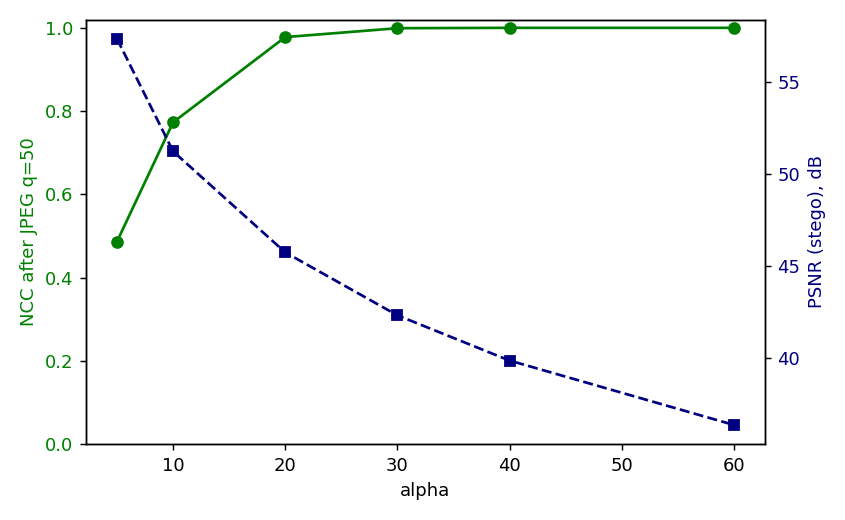
\includegraphics[width=0.7\textwidth,keepaspectratio]{images/ncc_vs_alpha_jpeg.png}
\caption{Зависимость NCC после JPEG-сжатия ($q = 50$) и PSNR стегоизображения от $\alpha$}
\end{figure}

% ================================================================
\section{Выводы о проделанной работе}

В работе реализован гибридный алгоритм встраивания цифрового водяного знака в частотную область изображения на основе сочетания дискретного косинусного преобразования и дискретного вейвлет-преобразования Хаара с перемешиванием ЦВЗ преобразованием Арнольда. Программа на Python обеспечивает встраивание ЦВЗ с расчётом метрик незаметности (PSNR, MSE, RMSE, SSIM) и неслепое извлечение ЦВЗ с расчётом метрик качества восстановления (BER, NCC). Корректность реализации подтверждена автоматической проверкой согласованности пары <<встраивание/извлечение>>.

По результатам вычислительных экспериментов сделаны следующие выводы:
\begin{enumerate}
    \item метод обеспечивает высокую незаметность встраивания: при параметрах по умолчанию ($\alpha = 20$) достигается $\mathrm{PSNR} = 45{,}75$~дБ и $\mathrm{SSIM} = 0{,}9949$ при точном восстановлении ЦВЗ в отсутствие атак;
    \item метод обладает выраженной робастностью к JPEG-сжатию: при $\alpha = 20$ ЦВЗ восстанавливается без ошибок вплоть до $q = 90$ и остаётся читаемым ($\mathrm{NCC} = 0{,}81$) даже при $q = 30$; алгоритм также устойчив к гауссовскому шуму и умеренно устойчив к масштабированию;
    \item наибольшую опасность для ЦВЗ представляют локальные искажения большой амплитуды (кадрирование, импульсный шум) и сдвиг яркости, искажающий DC-коэффициент полнокадрового ДКП;
    \item параметры алгоритма существенно влияют на показатели: коэффициент $\alpha$ задаёт компромисс между незаметностью и робастностью~--- его увеличение повышает устойчивость к атакам ценой снижения PSNR; при этом слишком малое $\alpha$ ($\le 5$) недопустимо, так как ЦВЗ теряется в шуме квантования пикселей уже без атак.
\end{enumerate}

Основным ограничением рассмотренного метода является \textit{неслепое} извлечение: для восстановления ЦВЗ необходимо исходное изображение-контейнер, что сужает область применения по сравнению со слепыми алгоритмами (например, алгоритмом межблочной разности коэффициентов ДКП~[1]). Тем не менее для задач подтверждения авторства и контроля целостности, где владелец располагает оригиналом, гибридный алгоритм ДКП+ДВП является эффективным и устойчивым решением.

\newpage
% ================================================================
\section{Список использованных источников}

\begin{enumerate}
    \item Ko H.-J., Huang C.-T., Horng G., Shiuh-Jeng W. Robust and blind image watermarking in DCT domain using inter-block coefficient correlation // Information Sciences.~--- 2020.~--- Vol.~517.~--- P.~128--147.
    \item Abdulrahman A.\,K., Ozturk S. A novel hybrid DCT and DWT based robust watermarking algorithm for color images // Multimedia Tools and Applications.~--- 2019.~--- Vol.~78, № 12.~--- P.~17027--17049.
    \item Конахович Г.\,Ф., Пузыренко А.\,Ю. Компьютерная стеганография. Теория и практика.~--- К.: МК-Пресс, 2006.~--- 288~с.
    \item Wang Z., Bovik A.\,C., Sheikh H.\,R., Simoncelli E.\,P. Image Quality Assessment: From Error Visibility to Structural Similarity // IEEE Transactions on Image Processing.~--- 2004.~--- Vol.~13, № 4.~--- P.~600--612.
    \item NumPy Documentation.~--- URL: \url{https://numpy.org/doc/} (дата обращения 10.06.2026).
    \item SciPy Documentation. Discrete Cosine Transforms.~--- URL: \url{https://docs.scipy.org/doc/scipy/reference/fft.html} (дата обращения 10.06.2026).
    \item scikit-image: Image processing in Python.~--- URL: \url{https://scikit-image.org} (дата обращения 10.06.2026).
    \item GitHub. Репозиторий с исходным кодом.~--- URL: \url{https://github.com/sikoslike-the-greatest/kriptoprak3} (дата обращения 10.06.2026).
\end{enumerate}

\end{document}
